\chapter{Circumvention Tools}
\section{Circumvention Tools}
Users who care about privacy and anonymity have options to increase their operational security and avoid censorship. Some of the most noteworthy tools are briefly explained below. It is worth mentioning that accessing these tools can be difficult for certain individuals. ProtonVPN discusses some of the countries that have outlawed VPN usage. \cite{protonvpn_vpn_legality_2} Some notable examples include Cuba, China, Vietnam and Egypt. This is a common theme; an arms race between oppressive regimes interested in censorship and circumvention and privacy based tools.

\textbf{Encryption}
Encryption is the fundamental security element driving communication over the internet. Bhanot describes encryption as "the process of converting normal data or plaintext to something incomprehensible or cipher-text by applying mathematical transformations or formulae." \cite{bhanot2015review} The importance of cryptography in security cannot be overstated. "Today, end-to-end encryption is the standard by which almost if not all communication over the internet occur. Examples of messaging platforms that offer this as standard include Telegram, Whatsapp and Facebook Messenger. CloudFlare states that end-to-end encryption "gives people total control over who can read their messages, enabling them to keep their messages private." \cite{cloudflare_e2ee} Encryption is the backbone of privacy online which allows users to leverage math to provide anonymity, at least in the best of cases. Zeadally, Das and Sklavos state the following about encryption "These techniques provide several security requirements, such as confidentiality, data integrity, entity authentication, message authentication, key management, non-repudiation, trustworthy data platforms, and digital signatures." \cite{ZEADALLY2021100075} It is clear from the research conducted that encryption has been fundamental in protecting user rights. 

\textbf{Transport Layer Security}
Transport Layer Security (TLS) is an example of encryption being used to secure data transfer online. TLS replaced the deprecated Secure Socket Layers (SSL), and TLS 1.3 is the standard by which data is transferred over the internet. According to the Internet Society, "TLS is normally implemented on top of TCP in order to encrypt Application Layer protocols such as HTTP, FTP, SMTP and IMAP." \cite{internetsociety_tls_basics} TLS operation is described in detail in RFC 8446 \cite{rfc8446} \cite{cloudflare_tls_handshake}. Below is a figure that shows a TLS handshake.

\begin{figure}
  \centering
  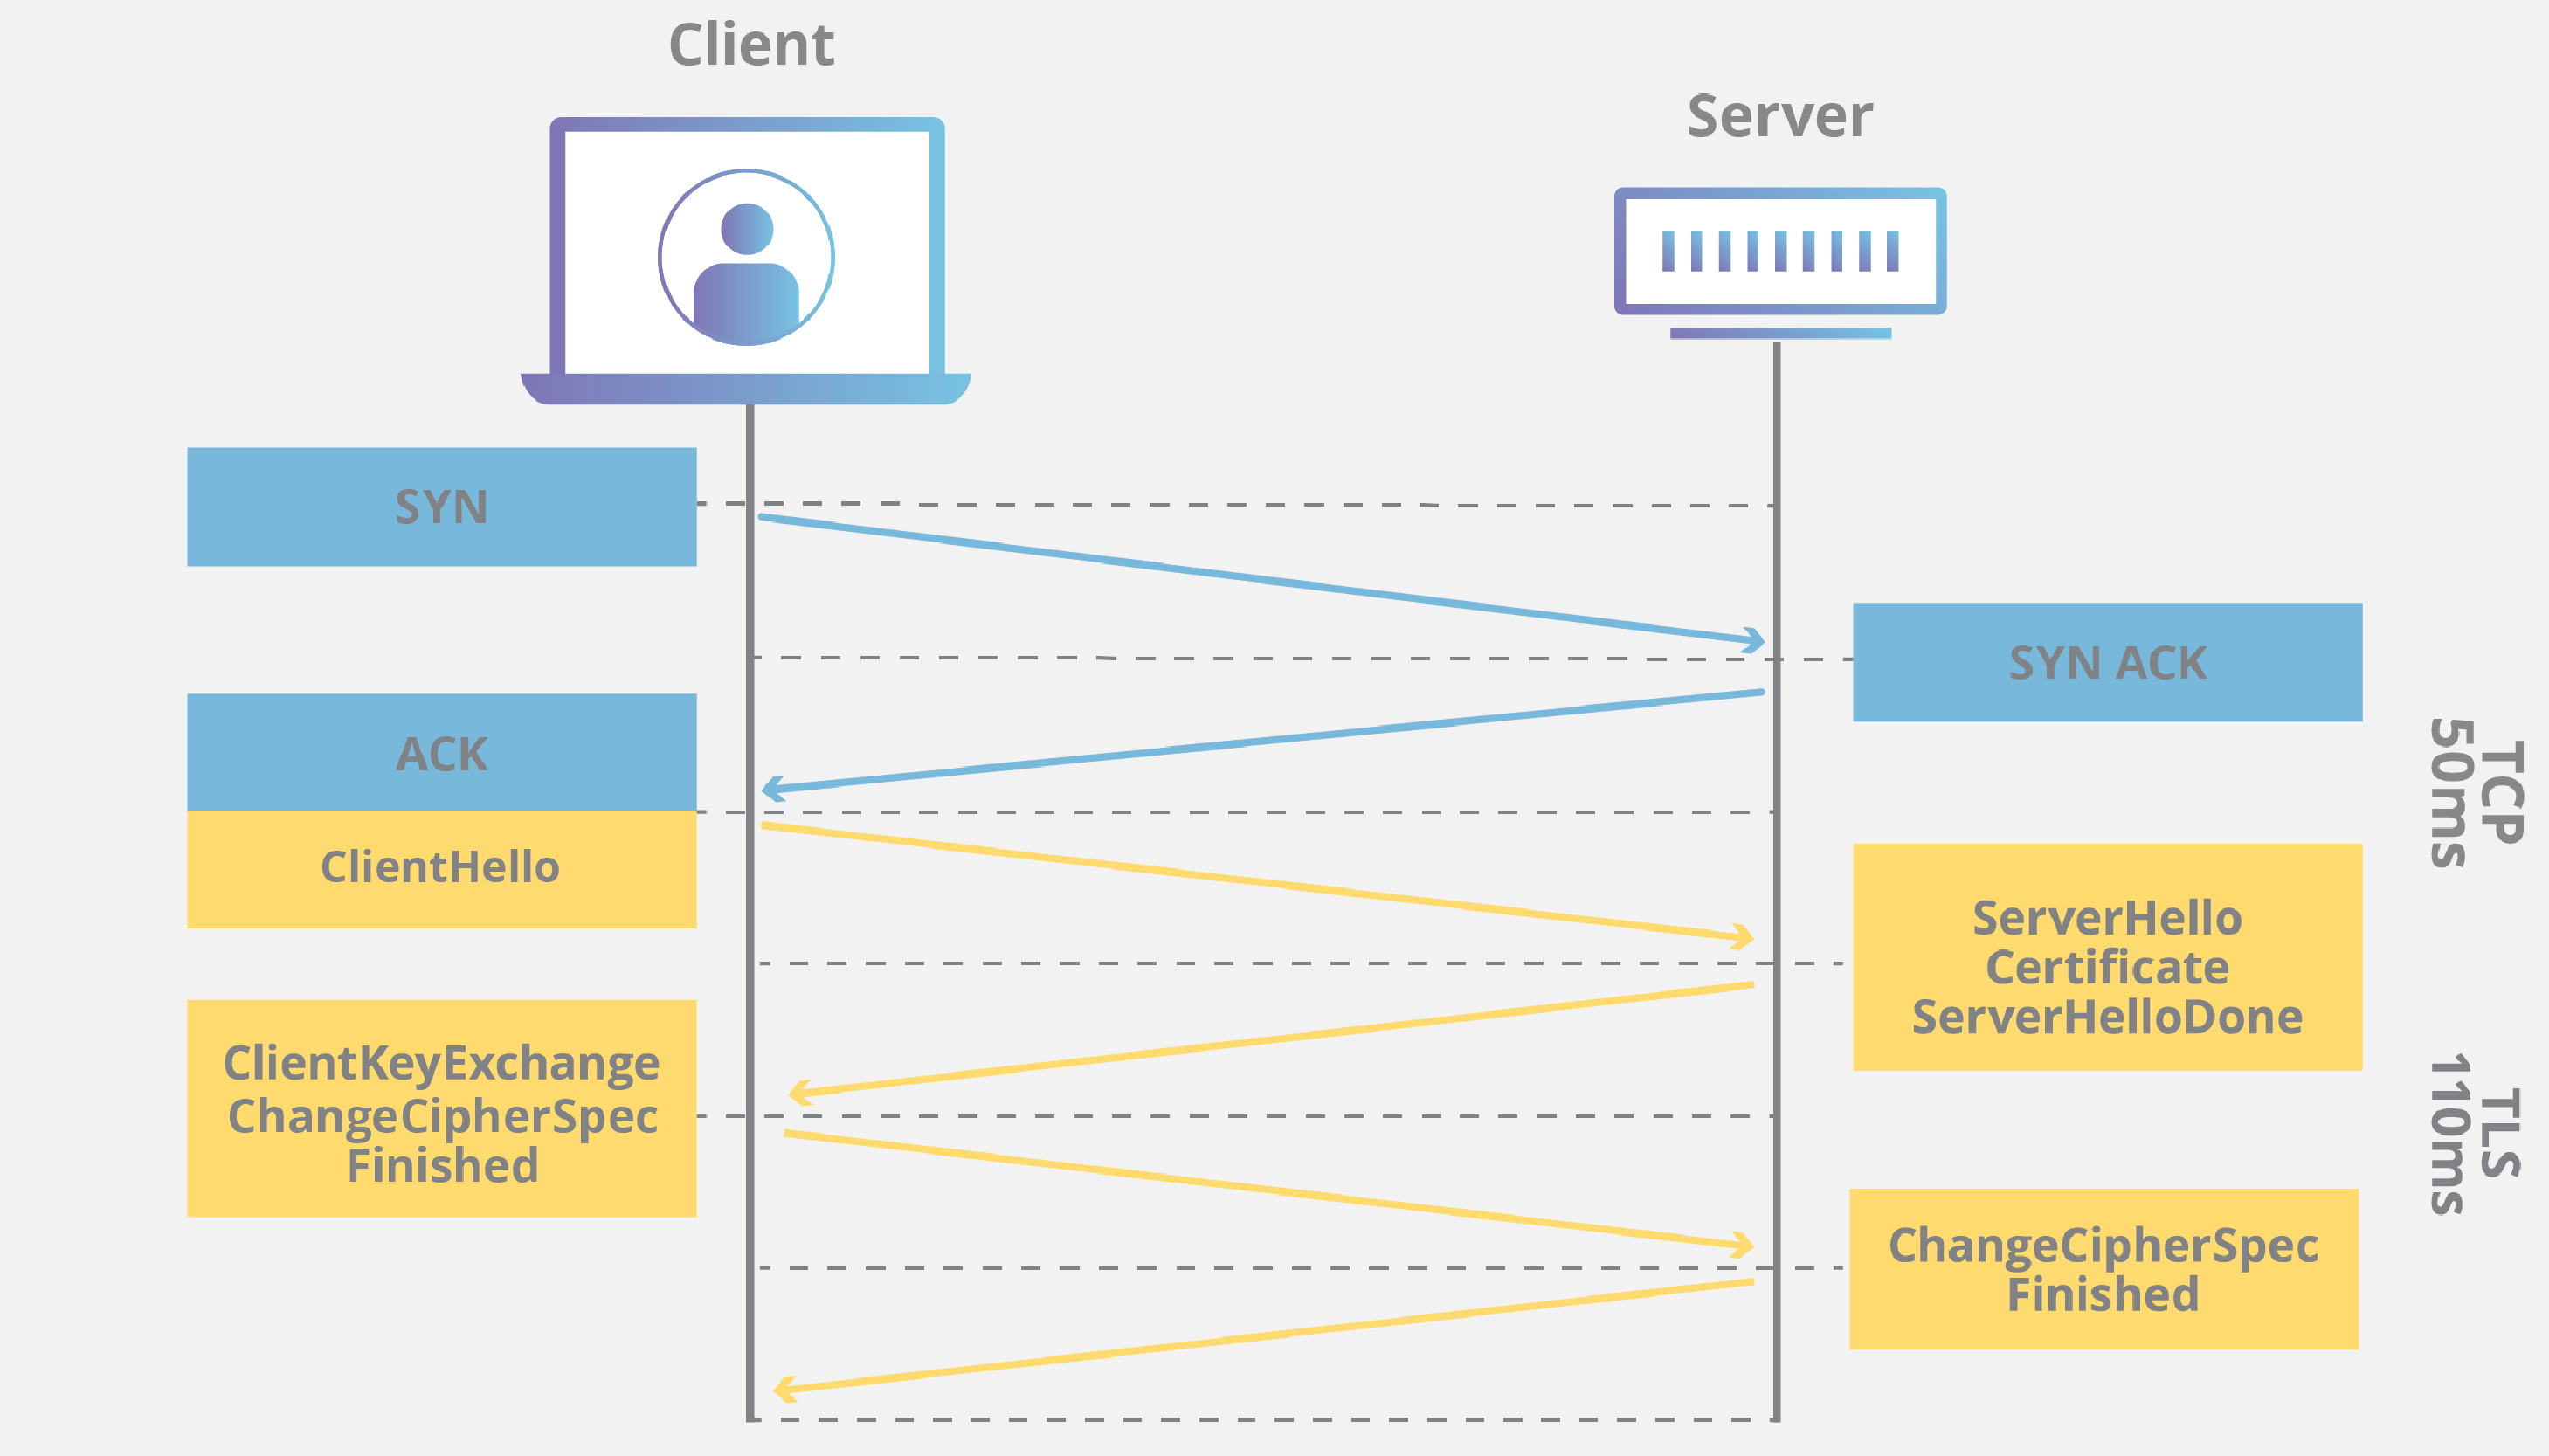
\includegraphics[width=\textwidth]{Circumvention Tools/TLS_Handshake.png}
  \caption{TLS Handshake, source https://www.cloudflare.com/en-gb/learning/ssl/what-happens-in-a-tls-handshake/}
  \label{fig:your_label_here}
\end{figure}

However, cryptography has not always had this virtuous reputation. The FBI lead what can only be described as a smear campaign against the technology in the early 2000s. In 1999, the director of the FBI, Louis Freeh, stated "encryption ultimately will devastate our ability to fight crime and prevent terrorism.” \cite{bitsbook_chapter5} Unsurprisingly, their stance has changed along with the growing necessity for encryption. Today, the FBI website states of encryption: "Law enforcement supports strong, responsibly managed encryption. This encryption should be designed to protect people’s privacy and also managed so U.S. tech companies can provide readable content in response to a lawful court order." \cite{fbi_lawful_access} The US government employs more methods than slander to defeat cryptography. The National Security Agency \cite{nsa_website} has a colourful reputation regarding its contributions to cryptographic standards. Dual\_EC\_DRBG was a cryptographic standard released by the NSA in 2007 and ratified by the National Institute of Standards and Technology (NIST). It was later found that this was insecure, having back door potential. CloudFlare defines a back door as "an intentional flaw in a cryptographic algorithm or implementation that allows an individual to bypass the security mechanism." \cite{cloudflare_nsa_backdoor} The discovery of this vulnerability is credited to Dan Shumow and Niels Ferguson. \cite{schneier_nsa_backdoor}

\textbf{Virtual Private Networks}
Virtual Private Networks (VPNs) are one of the most commonly used and important circumvention tools on the market. VPNs use tunnelling to encrypt packets at the lowest level, the OSI link layer. Microsoft developed Point-to-point Tunnelling Protocol (PPTP) which is now deprecated, having been shown to be insecure. \cite{microsoft_ptpt} More relevant examples of VPN protocols include IPsec \cite{rfc6071} and WireGuard \cite{wireguard_docs}. These protocols work by encapsulating packets and encrypting all of the information within. This provides secure data transfer over an insecure network. \cite{vpn_secure_connection2020} 

VPNs also allows users to effectively mask their IP address and change their apparent geo-location. This grants both privacy and circumvention potential; VPNs can be used to avoid geo - restrictions by routing traffic through more lenient countries. The role of VPNs in personal privacy and censorship circumvention cannot be overstated due to how commonplace the technology has become. According to SurfShark, a prominent provider, "over 1.6 billion people use VPNs." \cite{surfshark_vpn_users} Forbes states "Both the availability and usage of VPNs for personal use continue to rise," and this appears accurate. \cite{forbes_vpn_stats}

\textbf{The Onion Router (TOR)}
The Onion Router, originally developed by the US government, is an open-source network overlay that routes internet traffic through volunteer-operated relays. According to the founders, "Onion Routing is a distributed overlay network designed to anonymize TCP-based applications like web browsing, secure shell, and instant messaging." \cite{dingledine2004tor}

\begin{figure}
    \centering
    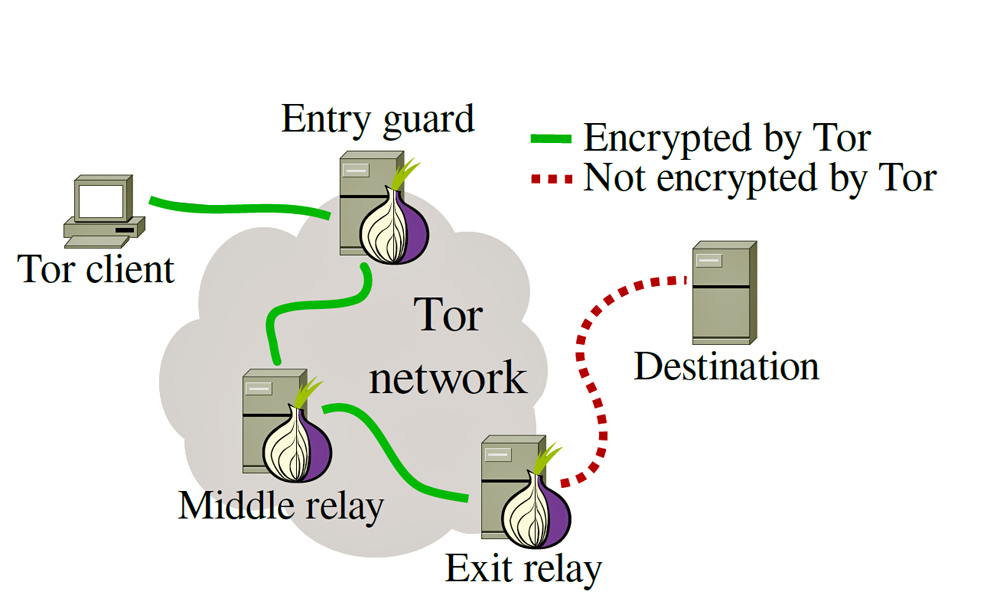
\includegraphics[width=1\linewidth]{HowTorWorks.png}
    \caption{How TOR works, source https://arstechnica.com/tech-policy/2014/07/report-rare-leaked-nsa-source-code-reveals-tor-servers-targeted/}
    \label{fig:enter-label}
\end{figure}

Requests travel through a relay passing three separate nodes. As a result, it is significantly more difficult to interpret the request’s origin and destination. Aside from granting privacy, Tor is also commonly used as a censorship circumvention method. Tor was believed to be secure for a long time but recent developments would suggest otherwise. \cite{tor_not_secure}

\textbf{TOR Bridges}
Previously, we have mentioned TOR relays and how three of them make up a circuit. The first hop over a relay is an important one; TOR bridges act as the first relay in certain circumstance. "Bridges are onion routers in the Tor Network whose IP addresses are not public." \cite{matic2017dissecting} Bridges act as a hidden and flexible way to access the TOR network. This allows individuals, (particulary in countries where TOR is heavily blocked), to bypass censorship, communicate securely and enhance privacy. For example, TOR bridges have been used to access TOR within China. \cite{dunna2018analyzing} \cite{cyberly_tor_blocked}


\textbf{Psiphon}
Psiphon is a "free and open-source Internet censorship circumvention tool that uses a combination of secure communication and obfuscation technologies." \cite{psiphon_guide} During the 2021 Cuban protests, the government shut down several social media sites. This lead to over 1 million protesters using Psiphon as a circumvention method. \cite{bloomberg_cubans_evade_internet} 

Typically, circumvention tools either divert web traffic so it avoids the machines that filter, or disguise the traffic as that that does not need to be filtered. Psiphon state on their website that "the Psiphon app has the ability to relay traffic through various communication protocols. It attempts to connect through different protocols until a connection is made." \cite{psiphon_guide} As previously mentioned, this technology has proved its value in combating internet censorship. 
